\documentclass{beamer}
\usepackage{tikz}
\usetikzlibrary{calc}
\usepackage{xcolor}
\usepackage{multicol}
\usepackage{amsmath}
\usepackage{amssymb}

% ================================================================
% Retrieval starters for a Year 10 mixed higher/foundation class,
% used across the algebraic fractions unit.
%
% Every starter draws on each of the three earlier topics: prime factor
% decomposition (factor trees, and HCF and LCM from Venn diagrams),
% indices (the index laws, negative and fractional indices) and surds
% (simplifying, adding, subtracting and multiplying). Each number skill
% is set beside the algebra it becomes once the fractions have letters
% in them. The five starters follow the order of the unit:
%
%   1  HCF and cancelling           -> simplifying single-term fractions
%   2  index laws                   -> dividing powers, negative indices
%   3  surds and single brackets    -> simplifying by factorising
%   4  double brackets              -> simplifying by factorising a quadratic
%   5  LCM and fraction arithmetic  -> adding, subtracting, multiplying
%                                      and dividing
%
% Within each starter the questions run from foundation to higher. A
% question marked (Extension) is higher tier, and the last question on
% each starter is a challenge that connects to the lesson.
% ================================================================

\setbeamertemplate{navigation symbols}{}
\setbeamersize{text margin left=0.4cm, text margin right=0.4cm}
\setlength{\multicolsep}{4pt}
\setlength{\columnsep}{20pt}

% ================================================================
% Answer-overlay helpers
% ================================================================
\newcommand{\ablank}[1]{%
  \alt<2>{\textcolor{red}{#1}}{\underline{\phantom{#1}}}%
}
\newcommand{\ashow}[1]{\uncover<2->{\textcolor{red}{\small #1}}}
\newcommand{\ashowq}[1]{\alt<2->{\textcolor{red}{\small #1}}{?}}

% Answers drawn straight on to a TikZ diagram, revealed on overlay 2 like \ashow.
% Space is reserved on overlay 1, so the diagram does not move between slides.
\usetikzlibrary{overlay-beamer-styles}
\tikzset{
  ans/.style     = {red, thick, visible on=<2->},
  ansfill/.style = {red!15, visible on=<2->},
  anslab/.style  = {red, font=\tiny, visible on=<2->},
}

% Used by the worked solutions rather than by this deck, so that each worked
% solution is first a question with room to write in and then the answer.
\newlength{\aworkpad}
\setlength{\aworkpad}{8mm}
\newcommand{\awork}[1]{%
  \par\vspace{\aworkpad}%
  \uncover<2->{#1}%
  \par\vspace{\aworkpad}%
}

% A gap drawn as a dotted box, for blanks inside a fraction or a chain of
% working. An \ablank underline sits on top of a fraction bar and reads as a
% second bar, so these gaps are boxed instead. The answer appears in red
% inside the box on overlay 2.
\newcommand{\abox}[1]{%
  \tikz[baseline=(b.base)]\node[draw=gray, densely dotted, inner sep=1.5pt] (b)
    {\alt<2->{\textcolor{red}{#1}}{\phantom{#1}}};%
}

% Every question list on these slides is tight, so that the diagram column and
% the question column both finish inside the slide.
\newcommand{\tightlist}{%
  \setlength{\itemsep}{0pt}\setlength{\parskip}{0pt}\setlength{\topsep}{0pt}%
}

% Factor trees. A composite number is written plainly and a prime is circled.
% The gaps are dotted: a box for a composite number and a circle for a prime.
\tikzset{
  tnum/.style   = {inner sep=1.5pt, font=\scriptsize},
  tprime/.style = {circle, draw, inner sep=0.5pt, minimum size=0.42cm, font=\scriptsize},
  tgap/.style   = {draw=gray, densely dotted, minimum width=0.5cm,
                   minimum height=0.36cm, inner sep=0pt},
  tpgap/.style  = {circle, draw=gray, densely dotted, minimum size=0.42cm, inner sep=0pt},
}

% Venn diagrams of prime factors, and the headings above each diagram.
% The set labels are anchored on the outside of each circle so that they
% stay clear of its edge however long the label is.
\tikzset{
  vleft/.style  = {thick, blue!60!black},
  vright/.style = {thick, orange!80!black},
  vlabl/.style  = {blue!60!black, anchor=east},
  vlabr/.style  = {orange!80!black, anchor=west},
  dhead/.style  = {font=\scriptsize\bfseries, anchor=west},
  vans/.style   = {anslab, font=\scriptsize},
}

\title{Algebraic Fractions: Starters}
\author{}
\date{}

\begin{document}

\frame{\titlepage}

%------------------------------------------------------------------
% STARTER 1: Prime factors, the HCF and cancelling
%------------------------------------------------------------------
\begin{frame}[t]{Starter 1: Prime Factors \& HCF}
\begin{columns}[T,onlytextwidth]

\column{0.36\textwidth}
\begin{center}
\vspace{-0.6em}
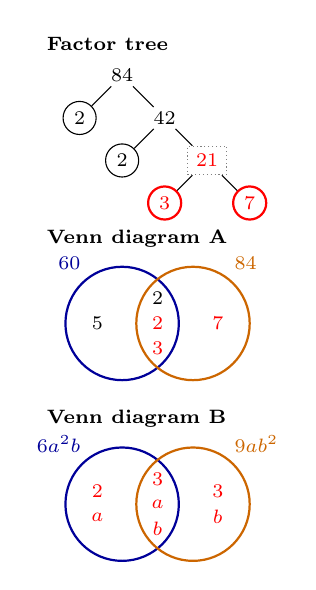
\begin{tikzpicture}[scale=0.9, every node/.style={font=\scriptsize}]

% ---- Factor tree for 84, with the lower branches to complete ----
\node[dhead] at (-1.2,0.45) {Factor tree};
\node[tnum]   (t84) at (0,0)       {$84$};
\node[tprime] (t2a) at (-0.6,-0.6) {$2$};
\node[tnum]   (t42) at (0.6,-0.6)  {$42$};
\node[tprime] (t2b) at (0,-1.2)    {$2$};
\node[tgap]   (t21) at (1.2,-1.2)  {};
\node[tpgap]  (t3)  at (0.6,-1.8)  {};
\node[tpgap]  (t7)  at (1.8,-1.8)  {};
\draw (t84) -- (t2a);  \draw (t84) -- (t42);
\draw (t42) -- (t2b);  \draw (t42) -- (t21);
\draw (t21) -- (t3);   \draw (t21) -- (t7);
% --- Q3 answer: the rest of the tree ---
\node[vans] at (t21) {$21$};
\node[tprime, ans] at (t3) {$3$};
\node[tprime, ans] at (t7) {$7$};

% ---- Venn diagram A: the prime factors of 60 and 84 ----
\begin{scope}[yshift=-3.5cm]
\node[dhead] at (-1.2,1.2) {Venn diagram A};
\draw[vleft]  (0,0)   circle (0.8);
\draw[vright] (1.0,0) circle (0.8);
\node[vlabl] at (-0.45,0.85) {$60$};
\node[vlabr] at (1.45,0.85)  {$84$};
\node at (-0.35,0)   {$5$};
\node at (0.5,0.35)  {$2$};
% --- Q4 answer: the other shared factors, and the 7 that only 84 has ---
\node[vans] at (0.5,0)     {$2$};
\node[vans] at (0.5,-0.35) {$3$};
\node[vans] at (1.35,0)    {$7$};
\end{scope}

% ---- Venn diagram B: the factors of 6a^2b and 9ab^2 ----
\begin{scope}[yshift=-6.05cm]
\node[dhead] at (-1.2,1.2) {Venn diagram B};
\draw[vleft]  (0,0)   circle (0.8);
\draw[vright] (1.0,0) circle (0.8);
\node[vlabl] at (-0.45,0.85) {$6a^2b$};
\node[vlabr] at (1.45,0.85)  {$9ab^2$};
% --- Q7 answer: 6a^2b = 2 x 3 x a x a x b and 9ab^2 = 3 x 3 x a x b x b ---
\node[vans] at (-0.35,0.18)  {$2$};
\node[vans] at (-0.35,-0.18) {$a$};
\node[vans] at (0.5,0.35)    {$3$};
\node[vans] at (0.5,0)       {$a$};
\node[vans] at (0.5,-0.35)   {$b$};
\node[vans] at (1.35,0.18)   {$3$};
\node[vans] at (1.35,-0.18)  {$b$};
\end{scope}

\end{tikzpicture}
\end{center}

\column{0.64\textwidth}
\vspace{-1.5em}
\footnotesize
\begin{enumerate}\tightlist
\begin{multicols}{2}
  \item Simplify $\sqrt{20}$.
        \ashow{$\sqrt{4\times5}=2\sqrt{5}$}
  \columnbreak
  \item Work out $2^{-1}$ and $9^{\frac12}$.
        \ashow{$\dfrac12$ and $3$}
\end{multicols}
  \item Complete the factor tree. Write $84$ as a product of prime factors in index form.
        \ashow{$84=2^2\times3\times7$}
  \item $60=2^2\times3\times5$. Complete Venn diagram A for $60$ and $84$, then find the
        HCF and the LCM of $60$ and $84$.
        \ashow{HCF $=12$; \; LCM $=2^2\times3\times5\times7=420$}
  \item Simplify $\dfrac{60}{84}$ by dividing by the HCF. Which numbers in Venn diagram A
        are not in the HCF?
        \ashow{$\dfrac{5}{7}$: the $5$ and the $7$, which are not shared}
  \item Simplify $\dfrac{x^5}{x^2}$ by writing out the $x$s and cancelling.
        \ashow{$x^2$ cancels from the top and the bottom, leaving $x^3=x^{5-2}$}
  \item (Challenge) Complete Venn diagram B for $6a^2b$ and $9ab^2$. Use it to simplify
        $\dfrac{6a^2b}{9ab^2}$.
        \ashow{The HCF is $3ab$, so $\dfrac{6a^2b}{9ab^2}=\dfrac{2a}{3b}$}
\end{enumerate}
\end{columns}
\end{frame}

%------------------------------------------------------------------
% STARTER 2: Index laws on cubes, cuboids and squares
%------------------------------------------------------------------
\begin{frame}[t]{Starter 2: Index Laws}
\begin{columns}[T,onlytextwidth]

\column{0.36\textwidth}
\begin{center}
\vspace{-0.6em}
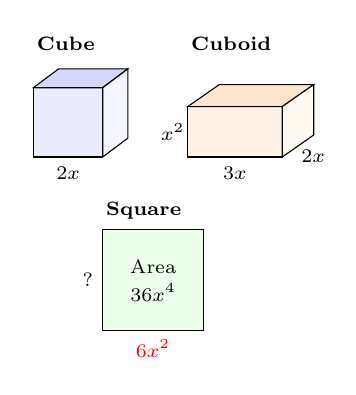
\begin{tikzpicture}[scale=0.8, every node/.style={font=\scriptsize}]

% ---- Cube with edge 2x ----
\node[dhead] at (-0.1,1.8) {Cube};
\draw[fill=blue!8]  (0,0) rectangle (1.1,1.1);
\draw[fill=blue!16] (0,1.1) -- (0.4,1.4) -- (1.5,1.4) -- (1.1,1.1) -- cycle;
\draw[fill=blue!4]  (1.1,0) -- (1.5,0.3) -- (1.5,1.4) -- (1.1,1.1) -- cycle;
\node[below] at (0.55,0) {$2x$};

% ---- Cuboid with edges 3x, x^2 and 2x ----
\begin{scope}[xshift=2.45cm]
\node[dhead] at (-0.1,1.8) {Cuboid};
\draw[fill=orange!10] (0,0) rectangle (1.5,0.8);
\draw[fill=orange!20] (0,0.8) -- (0.5,1.15) -- (2.0,1.15) -- (1.5,0.8) -- cycle;
\draw[fill=orange!5]  (1.5,0) -- (2.0,0.35) -- (2.0,1.15) -- (1.5,0.8) -- cycle;
\node[below] at (0.75,0) {$3x$};
\node[left, inner sep=1pt] at (0,0.4) {$x^2$};
\node[below right, inner sep=1pt] at (1.75,0.17) {$2x$};
\end{scope}

% ---- Square with area 36x^4 ----
\begin{scope}[xshift=1.1cm, yshift=-2.75cm]
\node[dhead] at (-0.1,1.9) {Square};
\draw[fill=green!8] (0,0) rectangle (1.6,1.6);
\node at (0.8,1.0)  {Area};
\node at (0.8,0.6)  {$36x^4$};
\node[left] at (0,0.8) {$?$};
% --- Q7 answer: the side length ---
\node[vans, below] at (0.8,0) {$6x^2$};
\end{scope}

\end{tikzpicture}
\end{center}

\column{0.64\textwidth}
\vspace{-1.5em}
\footnotesize
\begin{enumerate}\tightlist
\begin{multicols}{2}
  \item Write $72$ as a product of prime factors in index form.
        \ashow{$72=2^3\times3^2$}
  \columnbreak
  \item Simplify $\sqrt{8}+\sqrt{18}$.
        \ashow{$2\sqrt{2}+3\sqrt{2}=5\sqrt{2}$}
\end{multicols}
\begin{multicols}{2}
  \item Simplify $x^4\times x^3$ and $y^8\div y^2$.
        \ashow{$x^7$ and $y^6$}
  \columnbreak
  \item Write $2^{-3}$ and $x^{-2}$ as fractions.
        \ashow{$\dfrac18$ and $\dfrac{1}{x^2}$}
\end{multicols}
\begin{multicols}{2}
  \item Find the volume of the cube. Is it $2x^3$ or $8x^3$?
        \ashow{$(2x)^3=2^3x^3=8x^3$}
  \columnbreak
  \item Find the volume of the cuboid.
        \ashow{$3x\times2x\times x^2=6x^4$}
\end{multicols}
  \item The square has area $36x^4$, so its side length is $\left(36x^4\right)^{\frac12}$.
        Simplify this.
        \ashow{$36^{\frac12}\times x^{4\times\frac12}=6x^2$}
  \item (Extension) Complete the working.\\[2pt]
        \hspace*{1em}$8^{-\frac23}=\dfrac{1}{8^{\frac23}}=\dfrac{1}{\left(\sqrt[3]{8}\right)^2}
        =\dfrac{1}{\abox{$2$}^{\,2}}=\abox{$\dfrac14$}$
  \item (Challenge) Divide the volume of the cube by the volume of the cuboid. Write the
        answer as a fraction in its simplest form.
        \ashow{$\dfrac{8x^3}{6x^4}=\dfrac{4}{3x}$}
\end{enumerate}
\end{columns}
\end{frame}

%------------------------------------------------------------------
% STARTER 3: Surds, and factorising into a single bracket
%------------------------------------------------------------------
\begin{frame}[t]{Starter 3: Surds \& Single Brackets}
\begin{columns}[T,onlytextwidth]

\column{0.38\textwidth}
\begin{center}
\vspace{-0.6em}
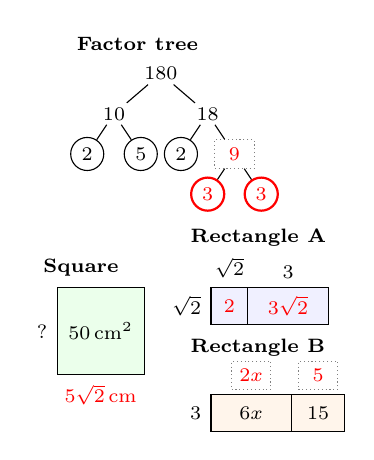
\begin{tikzpicture}[scale=0.85, every node/.style={font=\scriptsize}]

% ---- Factor tree for 180, with the right-hand branches to complete ----
% The 2 under 18 is given, so that 18 can only be split as 2 x 9.
\node[dhead] at (-1.4,0.45) {Factor tree};
\node[tnum]   (r)  at (0,0)        {$180$};
\node[tnum]   (a)  at (-0.7,-0.6)  {$10$};
\node[tnum]   (b)  at (0.7,-0.6)   {$18$};
\node[tprime] (a1) at (-1.1,-1.2)  {$2$};
\node[tprime] (a2) at (-0.3,-1.2)  {$5$};
\node[tprime] (b1) at (0.3,-1.2)   {$2$};
\node[tgap]   (b2) at (1.1,-1.2)   {};
\node[tpgap]  (c1) at (0.7,-1.8)   {};
\node[tpgap]  (c2) at (1.5,-1.8)   {};
\draw (r) -- (a);   \draw (r) -- (b);
\draw (a) -- (a1);  \draw (a) -- (a2);
\draw (b) -- (b1);  \draw (b) -- (b2);
\draw (b2) -- (c1); \draw (b2) -- (c2);
% --- Q3 answer: the rest of the tree ---
\node[vans] at (b2) {$9$};
\node[tprime, ans] at (c1) {$3$};
\node[tprime, ans] at (c2) {$3$};

% ---- Square with area 50 cm^2 ----
\begin{scope}[xshift=-1.55cm, yshift=-4.5cm]
\node[dhead] at (-0.35,1.6) {Square};
\draw[fill=green!8] (0,0) rectangle (1.3,1.3);
\node at (0.65,0.65) {$50$\,cm$^2$};
\node[left] at (0,0.65) {$?$};
% --- Q5 answer: the side length ---
\node[vans, below] at (0.65,0) {$5\sqrt{2}$\,cm};
\end{scope}

% ---- Rectangle A: sqrt2 (sqrt2 + 3). The sqrt2 by sqrt2 part is drawn square. ----
\begin{scope}[xshift=0.75cm, yshift=-3.75cm]
\node[dhead] at (-0.45,1.3) {Rectangle A};
\draw[fill=blue!6] (0,0) rectangle (0.55,0.55);
\draw[fill=blue!6] (0.55,0) rectangle (1.75,0.55);
\node[above] at (0.275,0.55) {$\sqrt{2}$};
\node[above] at (1.15,0.55)  {$3$};
\node[left]  at (0,0.275)    {$\sqrt{2}$};
% --- Q6 answer: the two areas ---
\node[vans] at (0.275,0.275) {$2$};
\node[vans] at (1.15,0.275)  {$3\sqrt{2}$};
\end{scope}

% ---- Rectangle B: factorising 6x + 15 ----
\begin{scope}[xshift=0.75cm, yshift=-5.35cm]
\node[dhead] at (-0.45,1.25) {Rectangle B};
\draw[fill=orange!8] (0,0) rectangle (1.2,0.55);
\draw[fill=orange!8] (1.2,0) rectangle (2.0,0.55);
\node[tgap] (bl) at (0.6,0.84) {};
\node[tgap] (br) at (1.6,0.84) {};
\node[left] at (0,0.275) {$3$};
\node at (0.6,0.275) {$6x$};
\node at (1.6,0.275) {$15$};
% --- Q7 answer: the missing lengths ---
\node[vans] at (bl) {$2x$};
\node[vans] at (br) {$5$};
\end{scope}

\end{tikzpicture}
\end{center}

\column{0.62\textwidth}
\vspace{-1.5em}
\footnotesize
\begin{enumerate}\tightlist
\begin{multicols}{2}
  \item Find the HCF of $18$ and $24$.
        \ashow{$6$}
  \columnbreak
  \item Work out $16^{\frac12}$ and $16^{-\frac12}$.
        \ashow{$4$ and $\dfrac14$}
\end{multicols}
  \item Complete the factor tree. Write $180$ as a product of prime factors in index form.
        \ashow{$180=2^2\times3^2\times5$}
  \item Use the prime factors to simplify $\sqrt{180}$.\\[1pt]
        \ashow{$\sqrt{2^2\times3^2\times5}=2\times3\times\sqrt{5}=6\sqrt{5}$}
  \item The square has area $50$\,cm$^2$. Find its side length as a simplified surd, and
        its perimeter.\\[1pt]
        \ashow{$\sqrt{50}=5\sqrt{2}$\,cm; \; $4\times5\sqrt{2}=20\sqrt{2}$\,cm}
  \item Complete rectangle A to expand $\sqrt{2}(\sqrt{2}+3)$.
        \ashow{$2+3\sqrt{2}$}
  \item Complete rectangle B to factorise $6x+15$. Then simplify $\dfrac{6x+15}{3}$.
        \ashow{$3(2x+5)$; \; $2x+5$, not $2x+15$}
  \item (Challenge) Sam says $\dfrac{6+\sqrt{18}}{3}=2+\sqrt{18}$. Explain Sam's mistake,
        then simplify it correctly.
        \ashow{Divide both terms by $3$: \; $2+\dfrac{3\sqrt{2}}{3}=2+\sqrt{2}$}
\end{enumerate}
\end{columns}
\end{frame}

%------------------------------------------------------------------
% STARTER 4: Double brackets as the sides of a rectangle
%------------------------------------------------------------------
\begin{frame}[t]{Starter 4: Double Brackets}
\begin{columns}[T,onlytextwidth]

\column{0.36\textwidth}
\begin{center}
\vspace{-0.6em}
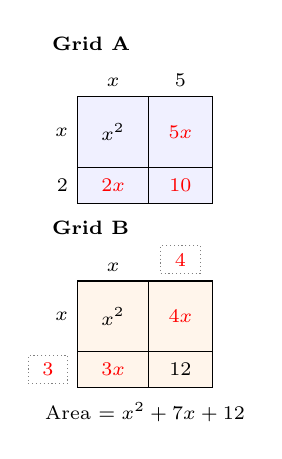
\begin{tikzpicture}[scale=0.9, every node/.style={font=\scriptsize}]

% ---- Grid A: (x + 2)(x + 5). The x by x part is drawn square. ----
\node[dhead] at (-0.5,0.75) {Grid A};
\draw[fill=blue!6] (0,0)      rectangle (1.0,-1.0);
\draw[fill=blue!6] (1.0,0)    rectangle (1.9,-1.0);
\draw[fill=blue!6] (0,-1.0)   rectangle (1.0,-1.5);
\draw[fill=blue!6] (1.0,-1.0) rectangle (1.9,-1.5);
\node[above] at (0.5,0)     {$x$};
\node[above] at (1.45,0)    {$5$};
\node[left]  at (0,-0.5)    {$x$};
\node[left]  at (0,-1.25)   {$2$};
\node at (0.5,-0.5) {$x^2$};
% --- Q3 answer: the other three areas ---
\node[vans] at (1.45,-0.5)  {$5x$};
\node[vans] at (0.5,-1.25)  {$2x$};
\node[vans] at (1.45,-1.25) {$10$};

% ---- Grid B: factorising x^2 + 7x + 12 ----
\begin{scope}[yshift=-2.6cm]
\node[dhead] at (-0.5,0.75) {Grid B};
\draw[fill=orange!8] (0,0)      rectangle (1.0,-1.0);
\draw[fill=orange!8] (1.0,0)    rectangle (1.9,-1.0);
\draw[fill=orange!8] (0,-1.0)   rectangle (1.0,-1.5);
\draw[fill=orange!8] (1.0,-1.0) rectangle (1.9,-1.5);
\node[above] at (0.5,0) {$x$};
\node[tgap] (gt) at (1.45,0.3) {};
\node[left]  at (0,-0.5) {$x$};
\node[tgap] (gl) at (-0.42,-1.25) {};
\node at (0.5,-0.5)   {$x^2$};
\node at (1.45,-1.25) {$12$};
\node[font=\scriptsize] at (0.95,-1.85) {Area $=x^2+7x+12$};
% --- Q5 answer: the missing lengths and areas ---
\node[vans] at (gt) {$4$};
\node[vans] at (gl) {$3$};
\node[vans] at (1.45,-0.5) {$4x$};
\node[vans] at (0.5,-1.25) {$3x$};
\end{scope}

\end{tikzpicture}
\end{center}

\column{0.64\textwidth}
\vspace{-1.5em}
\footnotesize
\begin{enumerate}\tightlist
\begin{multicols}{2}
  \item Is $3^{-2}$ equal to $-9$, $-6$ or $\frac19$?
        \ashow{$\dfrac{1}{3^2}=\dfrac19$}
  \columnbreak
  \item Simplify $\sqrt{50}-\sqrt{8}$. Is it $\sqrt{42}$?
        \ashow{No: $5\sqrt{2}-2\sqrt{2}=3\sqrt{2}$}
\end{multicols}
  \item Complete grid A to expand $(x+2)(x+5)$.
        \ashow{$x^2+7x+10$}
  \item Write $12$ as a product of prime factors, then list its factor pairs. Which pair
        adds to $7$?
        \ashow{$2^2\times3$; \; $1\times12$, $2\times6$, $3\times4$; \; $3+4=7$}
  \item Complete grid B to factorise $x^2+7x+12$.
        \ashow{$(x+3)(x+4)$, in either order}
  \item A rectangle has area $x^2+7x+12$ and width $x+3$. Find its length.
        Use this to simplify $\dfrac{x^2+7x+12}{x+3}$.\\[2pt]
        \ashow{$\dfrac{(x+3)(x+4)}{x+3}=x+4$}
  \item Factorise $x^2-9$. Use the difference of two squares to expand
        $(3+\sqrt{2})(3-\sqrt{2})$.
        \ashow{$(x+3)(x-3)$; \; $9-2=7$}
  \item (Challenge) $391=20^2-3^2$. Use this to write $391$ as a product of prime factors.
        \ashow{$(20+3)(20-3)=23\times17$, both prime}
\end{enumerate}
\end{columns}
\end{frame}

%------------------------------------------------------------------
% STARTER 5: The LCM as a common denominator, and the four operations
%------------------------------------------------------------------
\begin{frame}[t]{Starter 5: LCM \& Fractions}
\begin{columns}[T,onlytextwidth]

\column{0.36\textwidth}
\begin{center}
\vspace{-0.6em}
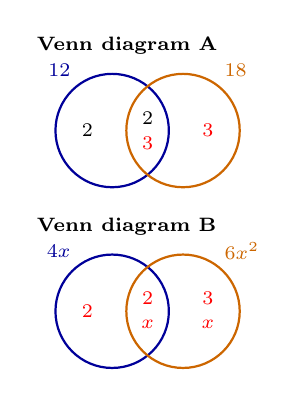
\begin{tikzpicture}[scale=0.9, every node/.style={font=\scriptsize}]

% ---- Venn diagram A: the prime factors of 12 and 18 ----
\node[dhead] at (-1.2,1.2) {Venn diagram A};
\draw[vleft]  (0,0)   circle (0.8);
\draw[vright] (1.0,0) circle (0.8);
\node[vlabl] at (-0.45,0.85) {$12$};
\node[vlabr] at (1.45,0.85)  {$18$};
\node at (-0.35,0)  {$2$};
\node at (0.5,0.18) {$2$};
% --- Q3 answer: the shared 3 and the 3 that only 18 has ---
\node[vans] at (0.5,-0.18) {$3$};
\node[vans] at (1.35,0)    {$3$};

% ---- Venn diagram B: the factors of 4x and 6x^2 ----
\begin{scope}[yshift=-2.55cm]
\node[dhead] at (-1.2,1.2) {Venn diagram B};
\draw[vleft]  (0,0)   circle (0.8);
\draw[vright] (1.0,0) circle (0.8);
\node[vlabl] at (-0.45,0.85) {$4x$};
\node[vlabr] at (1.45,0.85)  {$6x^2$};
% --- Q7 answer: 4x = 2 x 2 x x and 6x^2 = 2 x 3 x x x x ---
\node[vans] at (-0.35,0)     {$2$};
\node[vans] at (0.5,0.18)    {$2$};
\node[vans] at (0.5,-0.18)   {$x$};
\node[vans] at (1.35,0.18)   {$3$};
\node[vans] at (1.35,-0.18)  {$x$};
\end{scope}

\end{tikzpicture}
\end{center}

\column{0.64\textwidth}
\vspace{-1.5em}
\footnotesize
\begin{enumerate}\tightlist
\begin{multicols}{2}
  \item Simplify $a^3\times a^{-1}$.
        \ashow{$a^{3+(-1)}=a^2$}
  \columnbreak
  \item Work out $\sqrt{8}\times\sqrt{2}$.
        \ashow{$\sqrt{16}=4$}
\end{multicols}
  \item $12=2^2\times3$ and $18=2\times3^2$. Complete Venn diagram A, then find the HCF
        and the LCM of $12$ and $18$.
        \ashow{HCF $=6$; \; LCM $=2^2\times3^2=36$}
  \item Complete: \;
        $\dfrac{5}{12}+\dfrac{7}{18}=\dfrac{\abox{$15$}}{36}+\dfrac{\abox{$14$}}{36}
        =\dfrac{\abox{$29$}}{36}$
  \item Write $\dfrac{x}{12}-\dfrac{x}{18}$ as a single fraction.\\
        \ashow{$\dfrac{3x}{36}-\dfrac{2x}{36}=\dfrac{x}{36}$}
  \item Work out $\dfrac34\times\dfrac89$. Then simplify $\dfrac{3x}{4}\div\dfrac{9x}{10}$.\\
        \ashow{$\dfrac{24}{36}=\dfrac23$; \;
               $\dfrac{3x}{4}\times\dfrac{10}{9x}=\dfrac{30x}{36x}=\dfrac56$}
  \item $4x=2\times2\times x$ and $6x^2=2\times3\times x\times x$. Complete Venn diagram B,
        then find the LCM of $4x$ and $6x^2$.
        \ashow{$2\times2\times3\times x\times x=12x^2$}
  \item (Challenge) Write $\dfrac{5}{4x}+\dfrac{1}{6x^2}$ as a single fraction.
        \ashow{$\dfrac{15x}{12x^2}+\dfrac{2}{12x^2}=\dfrac{15x+2}{12x^2}$}
\end{enumerate}
\end{columns}
\end{frame}

\end{document}
